\documentclass[11pt,letterpaper]{article}
\usepackage[utf8]{inputenc}
\usepackage[T1]{fontenc}
\usepackage[spanish]{babel}
\usepackage{lmodern}
\usepackage{geometry}
\geometry{margin=2.35cm}
\usepackage{amsmath,amssymb,mathtools}
\usepackage{booktabs,longtable,tabularx,array}
\usepackage{xcolor,graphicx,float}
\usepackage{tikz}
\usetikzlibrary{arrows.meta,positioning,shapes.geometric,calc,fit}
\usetikzlibrary{babel}
\usepackage{fancyhdr}
\usepackage{hyperref}
\hypersetup{colorlinks=true,linkcolor=blue!45!black,urlcolor=blue!55!black,pdftitle={VotoSeguro - PIA de Criptografía}}
\usepackage{listings}
\definecolor{navy}{HTML}{173054}
\definecolor{bluea}{HTML}{2368AE}
\definecolor{pale}{HTML}{F1F6FC}
\definecolor{teal}{HTML}{168579}
\definecolor{grayb}{HTML}{5C697B}
\newcommand{\concepto}[1]{\textbf{\color{navy}#1}}
\newcommand{\code}[1]{\texttt{#1}}
\newcommand{\missingimage}[1]{\begin{center}\fcolorbox{bluea}{pale}{\parbox[c][2.2cm][c]{0.82\linewidth}{\centering\small\color{grayb}Evidencia pendiente: #1\\Captura auténtica al ejecutar en MacBook}}\end{center}}
\pagestyle{fancy}
\fancyhf{}
\fancyhead[L]{\small\textcolor{navy}{VotoSeguro -- PIA}}
\fancyhead[R]{\small\textcolor{grayb}{Criptografía aplicada}}
\fancyfoot[C]{\thepage}
\renewcommand{\headrulewidth}{0.4pt}
\setlength{\headheight}{15pt}
\setlength{\parindent}{0pt}
\setlength{\parskip}{6pt}
\setcounter{tocdepth}{2}
\lstset{basicstyle=\ttfamily\footnotesize,breaklines=true,frame=single,rulecolor=\color{gray!40},backgroundcolor=\color{pale},columns=fullflexible,showstringspaces=false}
\begin{document}
\begin{titlepage}
\centering
\vspace*{1.8cm}
{\Large\bfseries Proyecto Integrador de Aprendizaje\par}
\vspace{0.45cm}
{\color{bluea}\rule{0.82\linewidth}{2.2pt}\par}
\vspace{1.0cm}
{\Huge\bfseries\color{navy}VotoSeguro\par}
\vspace{0.32cm}
{\Large Sistema de Votación Electrónica Segura\par}
\vspace{.8cm}
{\large Prototipo académico para una elección municipal ficticia\par}
\vspace{.8cm}
\fcolorbox{bluea}{pale}{\parbox{0.83\linewidth}{\centering\vspace{7pt}\textbf{Modelo de amenaza definido por el docente}\\La autoridad electoral es honesta. Se estudia la protección frente a ataques externos.\\No se propone el uso de este software en elecciones reales.\vspace{7pt}}}
\vfill
\begin{tabular}{>{\bfseries}p{4cm}p{8cm}}
Alumno: & [Nombre completo]\\[5pt]
Matrícula: & [Matrícula]\\[5pt]
Materia: & Criptografía\\[5pt]
Docente: & [Nombre del docente]\\[5pt]
Institución: & [Institución]\\[5pt]
Entrega: & 14 de noviembre de 2026\\
\end{tabular}
\vfill
Monterrey, Nuevo León, México\\2026
\end{titlepage}
\tableofcontents\newpage
\section{Introducción y contexto}
La votación electrónica pretende permitir que ciudadanos expresen su preferencia electoral por medios informáticos. Sin embargo, un sistema electoral debe proteger datos sensibles sin perder la capacidad de comprobar que las operaciones autorizadas fueron registradas correctamente. Esta combinación plantea desafíos de confidencialidad, integridad, autenticación y auditabilidad.

Este trabajo presenta \textbf{VotoSeguro}, un prototipo local que simula una elección municipal con ciudadanos y candidaturas ficticios. La autoridad prepara el proceso, registra participantes de prueba, abre la urna, cierra la elección y publica un resultado firmado.

\subsection{Planteamiento del problema}
Un gobierno municipal hipotético requiere un mecanismo para que los electores registrados emitan un único voto desde un equipo conectado. Un atacante externo podría intentar robar credenciales, reemplazar mensajes cifrados, alterar registros o repetir envíos. Se busca minimizar estas amenazas mediante métodos criptográficos públicos y bibliotecas conocidas.

\subsection{Objetivo general}
Diseñar, implementar y evaluar un prototipo educativo de votación electrónica que combine autenticación de usuarios, cifrado híbrido de boletas, control transaccional de voto único, registros de integridad y firma digital de resultados.

\subsection{Objetivos específicos}
\begin{enumerate}
\item Proteger las contraseñas de las cuentas ficticias con Argon2id.
\item Cifrar en el navegador la selección mediante AES-256-GCM y RSA-OAEP.
\item Impedir múltiples votos por cuenta de forma atómica en SQLite.
\item Producir un comprobante de registro que no contenga la selección electoral.
\item Elaborar un registro encadenado mediante SHA-256 y firmar el resultado final con Ed25519.
\item Probar casos exitosos, datos inválidos, modificaciones deliberadas y solicitudes concurrentes.
\end{enumerate}

\subsection{Alcance y modelo de confianza}
\textbf{Supuesto esencial:} la autoridad electoral es honesta, administra correctamente las claves y no modifica intencionalmente la elección. El programa se orienta a demostrar resistencia frente a ciertos ataques \emph{externos}. No acredita anonimato absoluto, resistencia a coacción, seguridad del dispositivo del votante ni exactitud verificable universal del escrutinio. No utiliza votantes verdaderos ni datos de elecciones reales.

\subsection{Aporte del proyecto}
La parte original no consiste en inventar cifrados nuevos, sino en \emph{componer de manera justificada} algoritmos existentes dentro de un flujo coherente: autenticación, emisión, registro, auditoría y recuento.

\section{Requisitos del sistema y actores}
\subsection{Actores}
\begin{description}
\item[Ciudadano ficticio:] cuenta autorizada que accede, elige una opción y recibe un comprobante.
\item[Autoridad electoral honesta:] configura la elección, custodia las claves privadas, cierra la urna y ejecuta el escrutinio local.
\item[Atacante externo:] puede intentar enviar peticiones inválidas, manipular datos en tránsito o aprovechar credenciales robadas; no controla la autoridad ni las claves privadas.
\item[Observador:] consulta huellas de sobres cifrados y el manifiesto de resultados firmado.
\end{description}

\subsection{Requisitos funcionales}
\begin{longtable}{p{1.4cm}p{12.5cm}}
\toprule ID & Requisito\\ \midrule\endhead
RF-01 & Crear un padrón \emph{ficticio} de cuentas sin necesidad de servicios oficiales externos.\\
RF-02 & Comprobar usuario y contraseña, sin conservar esta última en texto claro.\\
RF-03 & Mostrar candidatos predefinidos y cifrar la elección localmente antes del envío.\\
RF-04 & Registrar a lo sumo un voto por cuenta mediante una actualización transaccional.\\
RF-05 & Emitir una huella SHA-256 del sobre cifrado sin incluir la candidatura elegida.\\
RF-06 & Registrar una cadena de huellas para detectar modificaciones.\\
RF-07 & Permitir cierre de urna y escrutinio offline de la autoridad honesta.\\
RF-08 & Generar resultados firmados y un listado de auditoría sin identidades.\\
\bottomrule
\end{longtable}

\subsection{Requisitos no funcionales}
\begin{itemize}
\item \concepto{Confidencialidad:} el servidor de votación ordinario no requiere conocer la clave privada para almacenar sobres.
\item \concepto{Integridad:} AES-GCM detecta alteraciones del contenido cifrado durante el escrutinio; SHA-256 y Ed25519 apoyan la integridad de la publicación.
\item \concepto{Autenticación:} se usan contraseñas verificadas con Argon2id y sesiones HTTP protegidas para el entorno local.
\item \concepto{Disponibilidad:} se aceptan limitaciones propias de SQLite y un único proceso de demostración.
\item \concepto{Mantenibilidad:} diseño por módulos, funciones pequeñas, pruebas y documentación.
\end{itemize}

\subsection{Criterios de aceptación}
\begin{enumerate}
\item Una cuenta válida puede emitir exactamente un voto y recibir un comprobante.
\item La misma cuenta no logra registrar un segundo voto aunque dos solicitudes lleguen simultáneamente.
\item Si se modifica un byte de la boleta cifrada, el descifrado autenticado falla.
\item Si un registro almacenado se altera, la auditoría detecta discrepancia.
\item Los resultados tienen una firma Ed25519 verificable.
\item Un observador no encuentra el nombre de usuario ni la candidatura en el registro público de huellas.
\end{enumerate}

\section{Especificación detallada de los protocolos}
\subsection{Parámetros criptográficos}
\begin{center}\small
\begin{tabularx}{\linewidth}{p{4cm}X}
\toprule Componente & Parámetros y función\\\midrule
RSA-OAEP & Par RSA de 3072 bits; OAEP con SHA-256 y MGF1-SHA-256; encapsula la clave AES.\\
AES-GCM & Clave aleatoria de 256 bits, nonce aleatorio de 96 bits y etiqueta de autenticación de 128 bits; protege el voto.\\
Argon2id & 19 MiB de memoria, dos iteraciones y paralelismo 1; verifica contraseñas con sal incorporada.\\
SHA-256 & Huellas hexadecimales de 256 bits de sobres cifrados y de la cadena.\\
Ed25519 & Firma del manifiesto final de escrutinio.\\
\bottomrule
\end{tabularx}
\end{center}

\subsection{Protocolo P0: preparación electoral}
\begin{enumerate}
\item La autoridad ejecuta \code{python manage.py init}; se generan claves RSA y Ed25519 de prueba.
\item Se crea la base SQLite con un padrón simulado de cinco cuentas, contraseñas aleatorias y hashes Argon2id.
\item La clave RSA \emph{pública} se entrega al navegador mediante \code{GET /api/config}. La clave privada permanece fuera del proceso web.
\item Se definen el identificador \code{MUNICIPAL-DEMO-2026} y las opciones A, B y C. La urna comienza en estado \code{open}.
\end{enumerate}
\textbf{Acuerdo de claves:} en este prototipo no se ejecuta Diffie--Hellman como aplicación propia. La clave simétrica se genera en cada navegador y se \emph{transporta protegida} mediante RSA-OAEP; TLS sería obligatorio para la autenticación del origen y la protección del canal en cualquier despliegue remoto.

\subsection{Protocolo P1: autenticación}
\begin{enumerate}
\item El usuario solicita el formulario de acceso y recibe un token anti-CSRF en una sesión firmada.
\item Envía usuario, contraseña y token anti-CSRF.
\item El servidor consulta el hash Argon2id del usuario y comprueba la contraseña. En éxito, renueva la sesión y limita su duración.
\item Se permite continuar a la boleta solamente si la sesión es válida y la elección está abierta.
\end{enumerate}
El hash Argon2id no es cifrado reversible de contraseña; es una función de derivación lenta resistente a ataques de adivinación \cite{owasp}.

\subsection{Protocolo P2: cifrado híbrido y emisión}
Sean $M$ la codificación JSON de la boleta, $K$ una clave AES aleatoria, $N$ un nonce y $A$ el identificador de elección usado como datos adicionales autenticados (AAD).
\begin{align}
K &\xleftarrow{\$}\{0,1\}^{256},\qquad N\xleftarrow{\$}\{0,1\}^{96},\\
(C,T)&=\operatorname{AES\text{-}GCM\text{-}Enc}(K,N,M,A),\\
W &= \operatorname{RSA\text{-}OAEP\text{-}Enc}(PK_{E},K).
\end{align}
El navegador transmite \code{wrapped\_key} $=W$, \code{nonce} $=N$ y \code{ciphertext} $=C\|T$, codificados en Base64. No transmite el nombre del candidato en texto claro dentro de esta petición.

El servidor comprueba la sesión, CSRF y tamaños del sobre. Inicia una transacción SQLite con \code{BEGIN IMMEDIATE}, actualiza \code{has\_voted} únicamente si era cero, guarda el sobre y confirma la transacción. Si la cuenta ya participó, rechaza la solicitud completa.

\subsection{Protocolo P3: comprobante y cadena de integridad}
Se calcula sobre una representación JSON canónica del sobre:
\begin{equation}
R_i=\operatorname{SHA256}(\operatorname{CanonicalJSON}(\text{election\_id},W_i,N_i,C_i\|T_i)).
\end{equation}
Con $H_0=00\ldots 00$ (64 caracteres hexadecimales):
\begin{equation}
H_i=\operatorname{SHA256}(H_{i-1}\,\|\,\texttt{:}\,\|\,i\,\|\,\texttt{:}\,\|\,R_i).
\end{equation}
La huella $R_i$ permite comprobar que un sobre aparece en la base de demostración. No contiene información de la candidatura en texto claro. Una cadena de hashes no constituye por sí misma una blockchain descentralizada.

\subsection{Protocolo P4: cierre, descifrado y escrutinio}
La autoridad cierra la urna y verifica los registros encadenados. Para cada sobre recupera:
\begin{align}
K&=\operatorname{RSA\text{-}OAEP\text{-}Dec}(SK_{E},W),\\
M&=\operatorname{AES\text{-}GCM\text{-}Dec}(K,N,C\|T,A).
\end{align}
Si falla la etiqueta, el JSON o la identificación electoral, se cuenta como boleta inválida. Si el candidato pertenece a las opciones predefinidas, su contador aumenta en una unidad.

\subsection{Protocolo P5: firma y verificación}
La autoridad construye un manifiesto $D$ con totales, número de votos válidos e inválidos, fecha UTC y último hash $H_n$. Calcula:
\begin{equation}
\sigma=\operatorname{Ed25519.Sign}(SK_{F},\operatorname{CanonicalJSON}(D)).
\end{equation}
Un tercero valida $\operatorname{Ed25519.Verify}(PK_F,D,\sigma)$. Esto verifica autoría e integridad de la \emph{publicación}; no prueba que la autoridad haya contado correctamente los votos, lo cual exigiría verificabilidad criptográfica adicional.

\subsection{Secuencia completa}
\begin{figure}[H]\centering
\resizebox{\linewidth}{!}{\begin{tikzpicture}[>=latex,font=\scriptsize,
part/.style={draw=bluea,rounded corners=2mm,fill=bluea!8,minimum width=3.2cm,minimum height=0.72cm,align=center},
msg/.style={-{Latex[length=2mm]},draw=navy,thick},
return/.style={-{Latex[length=2mm]},draw=teal,dashed,thick}]

\node[part] at (0,0) (a) {Ciudadano / navegador};
\node[part] at (5,0) (b) {Servidor Flask};
\node[part] at (10,0) (c) {SQLite};
\node[part] at (15,0) (d) {Autoridad (CLI)};

\foreach \x in {0,5,10,15}{\draw[gray,densely dashed] (\x,-.5)--(\x,-10.9);}

\draw[msg] (0,-1) -- node[above]{1. Credenciales + CSRF} (5,-1);
\draw[msg] (5,-1.7) -- node[above]{2. Consulta Argon2id} (10,-1.7);
\draw[return] (10,-2.2) -- node[above]{3. Resultado de hash} (5,-2.2);
\draw[return] (5,-2.7) -- node[above]{4. Sesión autenticada} (0,-2.7);
\draw[msg] (0,-3.5) -- node[above]{5. Consulta clave RSA pública} (5,-3.5);
\draw[return] (5,-4) -- node[above]{6. SPKI + elección} (0,-4);

\node[draw=teal,fill=teal!8,rounded corners,align=center] at (0,-4.9) {7. Genera AES + nonce\\ Cifra boleta y clave AES};

\draw[msg] (0,-5.8) -- node[above]{8. Sobre cifrado + CSRF} (5,-5.8);
\draw[msg] (5,-6.5) -- node[above]{9. UPDATE atómico + INSERT} (10,-6.5);
\draw[return] (10,-7) -- node[above]{10. Recibo SHA-256} (5,-7);
\draw[return] (5,-7.5) -- node[above]{11. Comprobante} (0,-7.5);
\draw[msg] (15,-8.3) -- node[above]{12. Cierra la elección} (10,-8.3);
\draw[msg] (15,-9.0) -- node[above]{13. Consulta sobres cifrados} (10,-9.0);
\draw[return] (10,-9.5) -- node[above]{14. Sobres + cadena} (15,-9.5);

\node[draw=teal,fill=teal!8,rounded corners,align=center] at (15,-10.25) {15. Descifra / cuenta / firma\\ manifiesto con Ed25519};

\end{tikzpicture}
}
\caption{Intercambio entre votante, web, base de datos y autoridad honesta.}
\end{figure}

\section{Diseño e implementación del software}
\subsection{Arquitectura modular}
\begin{figure}[H]\centering
\resizebox{\linewidth}{!}{\begin{tikzpicture}[>=latex,font=\small,
box/.style={draw=bluea,rounded corners=3mm,fill=bluea!7,minimum width=3.8cm,minimum height=1.7cm,align=center},
dat/.style={draw=teal,rounded corners=2mm,fill=teal!8,minimum width=4.2cm,minimum height=1.5cm,align=center},
arrow/.style={-{Latex[length=3mm]},thick,draw=navy}]

\node[box] (web) at (0,0) {\textbf{Navegador del votante}\\ HTML / JavaScript\\ Web Crypto API};
\node[box] (flask) at (6.0,0) {\textbf{Aplicación Flask}\\ sesión / Argon2id / CSRF\\ API de voto};
\node[dat] (voters) at (12.4,1.7) {\textbf{SQLite: voters}\\ usuario / hash Argon2id\\ marca de participación};
\node[dat] (ballots) at (12.4,-1.7) {\textbf{SQLite: ballots}\\ sobres cifrados / huellas\\ cadena SHA-256};
\node[box] (authority) at (18.9,-1.7) {\textbf{Autoridad honesta}\\ CLI: cierre / escrutinio\\ RSA privada / Ed25519};


\draw[arrow] (web) -- node[above,align=center]{HTTP local + CSRF\\sobre cifrado} (flask);
\draw[arrow] (flask) -- (voters);
\draw[arrow] (flask) -- (ballots);
\draw[arrow] (ballots) -- node[above]{lectura offline} (authority);
\draw[arrow,dashed] (authority.south) -- ++(0,-1.2) -| node[below,pos=.25]{resultados firmados y auditoría} (flask.south);

\node[draw=grayb,fill=gray!7,rounded corners=2mm,align=center,font=\footnotesize] at (10.2,-4.4) {Clave \textbf{pública} RSA en el navegador; clave \textbf{privada} solamente en el escrutinio local.\\ Las dos tablas SQLite comparten el mismo archivo físico: no existe anonimato fuerte.};

\end{tikzpicture}
}
\caption{Arquitectura lógica. El almacén SQLite contiene dos tablas separadas, no dos servidores independientes.}
\end{figure}

\subsection{Lenguajes y tecnologías}
\begin{longtable}{p{3.0cm}p{10.8cm}}
\toprule Tecnología & Justificación técnica\\\midrule\endhead
Python 3 & Facilita pruebas, modularidad e integración con bibliotecas de criptografía revisadas.\\
Flask & Rutas de aplicación web sencillas, sesiones firmadas y plantillas Jinja2.\\
JavaScript + Web Crypto & Cifra dentro del navegador; la selección no viaja en texto claro dentro del cuerpo de la petición. Web Crypto requiere un contexto seguro (HTTPS o localhost) \cite{mdn}.\\
SQLite & Almacenamiento transaccional de uso único y control de concurrencia mediante \code{BEGIN IMMEDIATE}.\\
\code{cryptography} & Implementaciones RSA-OAEP, AES-GCM y Ed25519 sin escribir primitivas manualmente.\\
\code{argon2-cffi} & Implementación Argon2id para almacenar hashes de contraseñas.\\
Pytest & Automatiza comprobación de casos normales, inválidos y concurrentes.\\
LaTeX y TikZ & Documentación reproducible con fórmulas y diagramas vectoriales editables.\\
\bottomrule
\end{longtable}

\subsection{Estructura de archivos}
\begin{center}\small
\begin{tabularx}{\linewidth}{p{5cm}X}
\toprule Archivo & Función\\\midrule
\code{app.py} & Rutas HTTP, autorización por sesión y protección CSRF.\\
\code{launcher.py} & Arranque web local en \code{127.0.0.1:5000}.\\
\code{manage.py} & Inicializar, cerrar, escrutar y verificar desde terminal.\\
\code{src/votoseguro/config.py} & Identificador electoral, candidatos y constantes.\\
\code{src/votoseguro/crypto.py} & Claves RSA, Ed25519, AES-GCM y funciones SHA-256.\\
\code{src/votoseguro/storage.py} & SQLite, voto único y cadena hash.\\
\code{src/votoseguro/services.py} & Argon2id, autenticación, auditoría y escrutinio.\\
\code{static/vote.js} & Cifrado de boleta con Web Crypto API en el cliente.\\
\code{templates/*.html} & Acceso, elección, comprobante, auditoría y resultados.\\
\code{tests/test\_election.py} & Pruebas de integridad y comportamiento de los protocolos.\\
\bottomrule
\end{tabularx}
\end{center}

\subsection{Base de datos y separación lógica}
La tabla \code{voters(username, password\_hash, has\_voted)} almacena credenciales de prueba y participación. La tabla \code{ballots} almacena sobres cifrados, nonces y hashes de integridad sin incluir el identificador del votante. \code{settings} conserva el estado abierto/cerrado.

\textbf{Limitación:} aunque no existe una columna explícita que relacione votante y selección, el mismo sistema web sigue observando autenticaciones, solicitudes y tiempos. Sin tecnologías de credenciales ciegas, redes anónimas y controles adicionales, no se garantiza desvinculación criptográfica fuerte.

\subsection{Pseudocódigo del registro de voto}
\begin{lstlisting}
FUNCION registrar_voto(usuario, sobre):
    validar_estructura(sobre)
    comenzar_transaccion_inmediata()
    SI eleccion_cerrada(): RECHAZAR
    SI actualizar_votante_si_no_voto(usuario) != 1:
        RECHAZAR
    recibo = SHA256(JSON_canonico(sobre))
    anterior = ultimo_hash_o_genesis()
    cadena = SHA256(anterior || indice || recibo)
    guardar_sobre(sobre, recibo, anterior, cadena)
    CONFIRMAR_TRANSACCION
    RETORNAR recibo
FIN FUNCION
\end{lstlisting}
\subsection{Diagrama de flujo: emisión}
\begin{figure}[H]\centering
\resizebox{0.85\linewidth}{!}{\begin{tikzpicture}[>=latex,font=\small,node distance=0.6cm,
boxstep/.style={rectangle,draw=bluea,fill=bluea!7,rounded corners=2mm,text width=6cm,align=center,minimum height=.85cm},
decision/.style={diamond,draw=teal,fill=teal!8,aspect=2.6,text width=3.5cm,align=center,inner sep=1pt},
edge/.style={-{Latex[length=2.5mm]},thick,draw=navy}]

\node[boxstep] (start) {Inicio: solicitar boleta};
\node[decision,below=of start] (login) {¿Sesión y CSRF válidos?};
\node[boxstep,below=0.95cm of login] (enc) {En el navegador: generar clave AES y nonce; cifrar con AES-GCM y RSA-OAEP};
\node[boxstep,below=of enc] (db) {Enviar sobre cifrado e iniciar transacción SQLite inmediata};
\node[decision,below=0.7cm of db] (elig) {¿Cuenta sin voto previo y elección abierta?};
\node[boxstep,below=1.1cm of elig] (save) {Marcar participación, guardar sobre y calcular cadena SHA-256};
\node[boxstep,below=of save] (end) {Confirmar transacción y devolver comprobante};
\node[boxstep,right=2.7cm of login] (reject1) {Rechazar solicitud};
\node[boxstep,right=2.7cm of elig] (reject2) {Deshacer transacción y rechazar};

\draw[edge] (start)--(login);
\draw[edge] (login)--node[right]{sí}(enc);
\draw[edge] (login.east)--node[above]{no}(reject1.west);
\draw[edge] (enc)--(db);
\draw[edge] (db)--(elig);
\draw[edge] (elig)--node[right]{sí}(save);
\draw[edge] (elig.east)--node[above]{no}(reject2.west);
\draw[edge] (save)--(end);

\end{tikzpicture}
}
\caption{Validación de la sesión, cifrado local, transacción atómica y emisión del recibo.}
\end{figure}

\subsection{Instrucciones de uso}
\textbf{Para MacOS}
\begin{lstlisting}
python3 -m venv .venv
source .venv/bin/activate
python -m pip install -r requirements.txt
python manage.py init
python launcher.py
# Abrir http://127.0.0.1:5000/login

# En otra terminal, al concluir:
python manage.py close
python manage.py tally
python manage.py verify
python -m pytest -q
\end{lstlisting}

\newpage
\textbf{Para Windows}
\begin{lstlisting}
#1. Construir el entorno virtual
py -m venv .venv

#2. Activarlo
.\.venv\Scripts\Activate.ps1

#3. Instalar las bibliotecas (Si es la primera vez que se ejecuta)
python -m pip install -r requirements.txt

#4. Inicializar la urna
python manage.py init

#5. Iniciar el servidor
python launcher.py

#6. Abrir en el navegador (preferiblemente Chrome) http://127.0.0.1:5000/login
bruh...
por definir
\end{lstlisting}
Los comandos administrativos se ejecutan \emph{localmente}; no se expone un botón web para cerrar o escrutar. 

\section{Selección de métodos, seguridad y escalabilidad}
\subsection{Justificación de algoritmos}
\begin{longtable}{p{2.4cm}p{4.3cm}p{6.1cm}}
\toprule Método & Ventaja para el caso & Limitaciones y razones de selección\\\midrule\endhead
AES-256-GCM & Cifrado autenticado veloz para una boleta pequeña & Se debe usar un nonce distinto para cada cifrado con la misma clave; aquí cada voto genera una clave AES nueva y nonce aleatorio.\\
RSA-OAEP & Protege una clave AES corta con la clave pública de la autoridad & Tamaño de clave y operaciones más costosos que la criptografía simétrica; se elige para enseñar cifrado híbrido.\\
Argon2id & Resiste mejor ataques de adivinación que los hashes rápidos & Tiene costo de memoria y CPU ajustable; no elimina robo de credenciales ni phishing.\\
SHA-256 & Huella determinista con resistencia a colisiones conocida & No es una firma ni ofrece secreto; una cadena no evita que su propietario reescriba la historia sin un ancla externa.\\
Ed25519 & Firma compacta y verificación eficiente & No cifra, ni demuestra la corrección de los votos contados.\\
\bottomrule
\end{longtable}

\subsection{Modelo de amenazas}
\begin{longtable}{p{3.5cm}p{5.4cm}p{4.2cm}}
\toprule Amenaza externa & Control implementado & Riesgo residual\\\midrule\endhead
Cambio de voto cifrado & AES-GCM valida etiqueta y AAD en escrutinio & El cambio puede ser almacenado antes de descubrirse; se marca inválido.\\
Doble envío concurrente & Actualización condicional en SQLite con transacción inmediata & Cuentas falsas si el padrón inicial no es confiable.\\
Contraseña robada & Hash Argon2id y sesiones con CSRF & No evita suplantación cuando el atacante conoce la contraseña.\\
Alteración de registro & Cadena SHA-256; manifiesto firmado después del cierre & Antes del cierre la autoridad honesta sigue siendo una premisa esencial.\\
Suplantación del servidor & No se modela en localidad; para red real es obligatorio TLS autenticado & Si el código JS servido es malicioso, puede revelar el voto.\\
Exposición de claves & El servidor web sólo carga la clave pública; privada en ruta local & Sin HSM; usuario del sistema con privilegios puede leer claves.\\
DoS / sobrecarga & Límite de tamaño HTTP, SQLite para práctica local & Sin balanceador ni anti-DDoS; capacidad limitada.\\
\bottomrule
\end{longtable}

\subsection{Privacidad, transparencia y verificabilidad}
Se separa \emph{lógicamente} la lista de votantes de los sobres cifrados. Los comprobantes y registros públicos muestran hashes de sobres, no el nombre de usuario o la elección. El observador puede revisar la cadena y firma final; ello permite detectar ciertas alteraciones, pero \textbf{no prueba} que el contenido cifrado fue descifrado correctamente ni que todos los ciudadanos votaron libremente. Según los principios VVSG, la confidencialidad del voto, protección de datos y verificabilidad son objetivos independientes \cite{nistvvsg}.

\subsection{Por qué no usar blockchain}
Se decidió usar una cadena SHA-256 más firma final. Una blockchain es más que una secuencia de hashes: requiere consenso, reglas de participación y un modelo de confianza distribuida. Como el escenario presupone una autoridad electoral honesta, no se necesita incorporar consenso para demostrar cifrado, integridad y registro. La propuesta tampoco debe confundirse con una elección públicamente verificable de extremo a extremo.

\subsection{Escalabilidad}
SQLite es adecuada para pruebas locales y pequeñas cantidades de votos. En un escenario municipal real habría que migrar a una base de datos transaccional escalable, separar servicios, usar colas y monitoreo, gestionar claves en HSM, diseñar un protocolo de anonimato verificable y contar con auditorías independientes y mecanismos antifraude. La interfaz es adaptable a móviles, pero no se ha realizado una prueba de carga municipal.

\subsection{Criptografía postcuántica como trabajo futuro}
RSA y Ed25519 pertenecen a la criptografía de clave pública clásica, no resistente a una computadora cuántica criptográficamente relevante. Una evolución podría estudiar ML-KEM y ML-DSA, pero migrar requeriría rediseñar el protocolo y reevaluar rendimiento y seguridad; no se afirma que esta versión sea postcuántica.

\section{Plan de verificación, resultados y evidencias}
\subsection{Pruebas de módulo ejecutadas}
Se diseñaron pruebas unitarias sobre la lógica criptográfica y la persistencia; se ejecutaron en el entorno de preparación del proyecto. Resultado observado: \textbf{20 pruebas aprobadas}. Entre los casos están los siguientes:

\begin{longtable}{p{4.2cm}p{8.9cm}}
\toprule Caso & Resultado esperado\\\midrule\endhead
Inicio de sesión correcto e incorrecto & Aceptar sólo la contraseña que verifica el hash Argon2id.\\
Reversibilidad AES + RSA & Descifrar la misma candidatura que fue cifrada.\\
Manipular ciphertext o nonce & Rechazo por error de autenticación AES-GCM.\\
Sobre inválido & Rechazo por estructura, Base64 o tamaños incorrectos.\\
Dos votos con una misma cuenta & Aceptar primero, rechazar segundo.\\
Dos envíos concurrentes & Solamente una transacción exitosa.\\
Cuenta inexistente & El sistema rechaza el intento.\\
Modificar tabla de boletas & Auditoría de cadena falla.\\
Cierre de elección & No se aceptan más votos.\\
Tally y firma & Se cuentan 2 votos A, 1 B, 0 C y se valida Ed25519.\\
Alterar conteos firmados & La verificación de firma falla.\\
Cambio de la cadena publicada & La auditoría devuelve falso.\\
Cifrado JS/Python & Una boleta cifrada con Web Crypto (Node) es descifrable en Python.\\
\bottomrule
\end{longtable}

\subsection{Demostración de escrutinio desde la terminal}
En una ejecución aislada con tres cuentas de prueba, se registraron las selecciones A, C y A; después de cerrar la elección, el programa generó un resultado de \textbf{2 votos para A, 0 para B y 1 para C}, sin boletas inválidas. La verificación de la firma Ed25519 y de la cadena devolvió un estado válido. Esta ejecución corresponde a datos ficticios generados para la validación del software.


\subsection{Capturas}
\textbf{> Inicio de sesión}
\newline
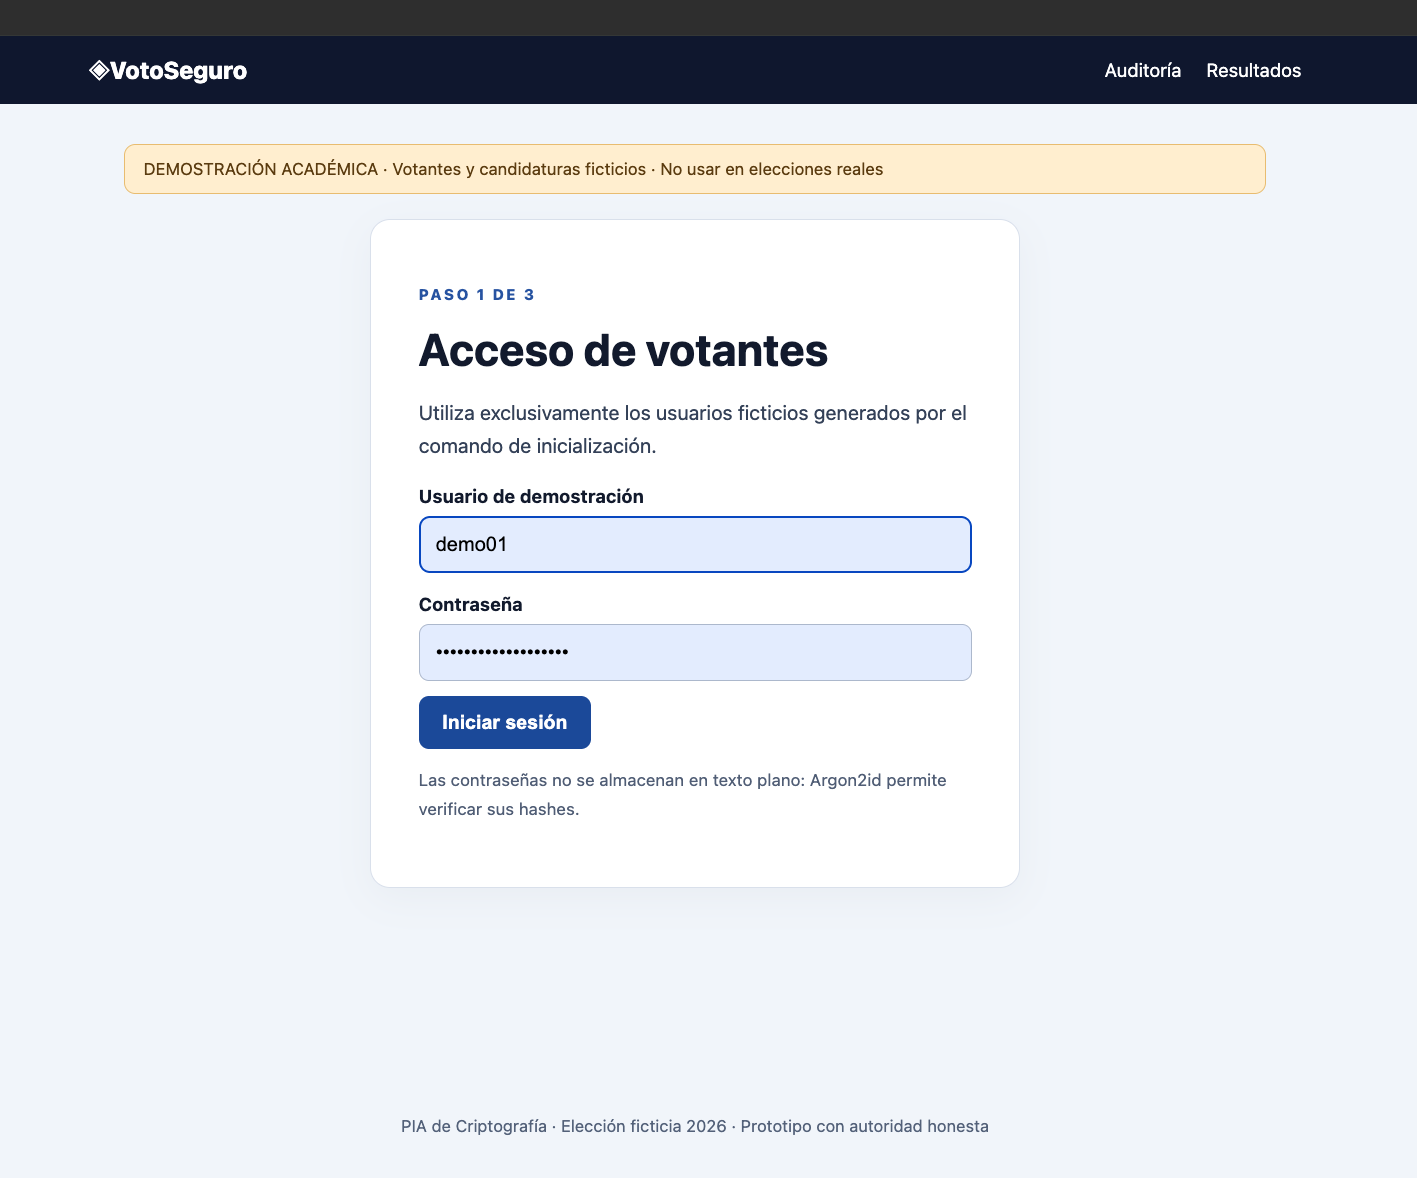
\includegraphics[width=.85\linewidth]{docs/evidencias/Formulario de inicio de sesión con usuario ficticio.png}

\newpage
\textbf{Menú de selección (3 candidatos)}
\newline
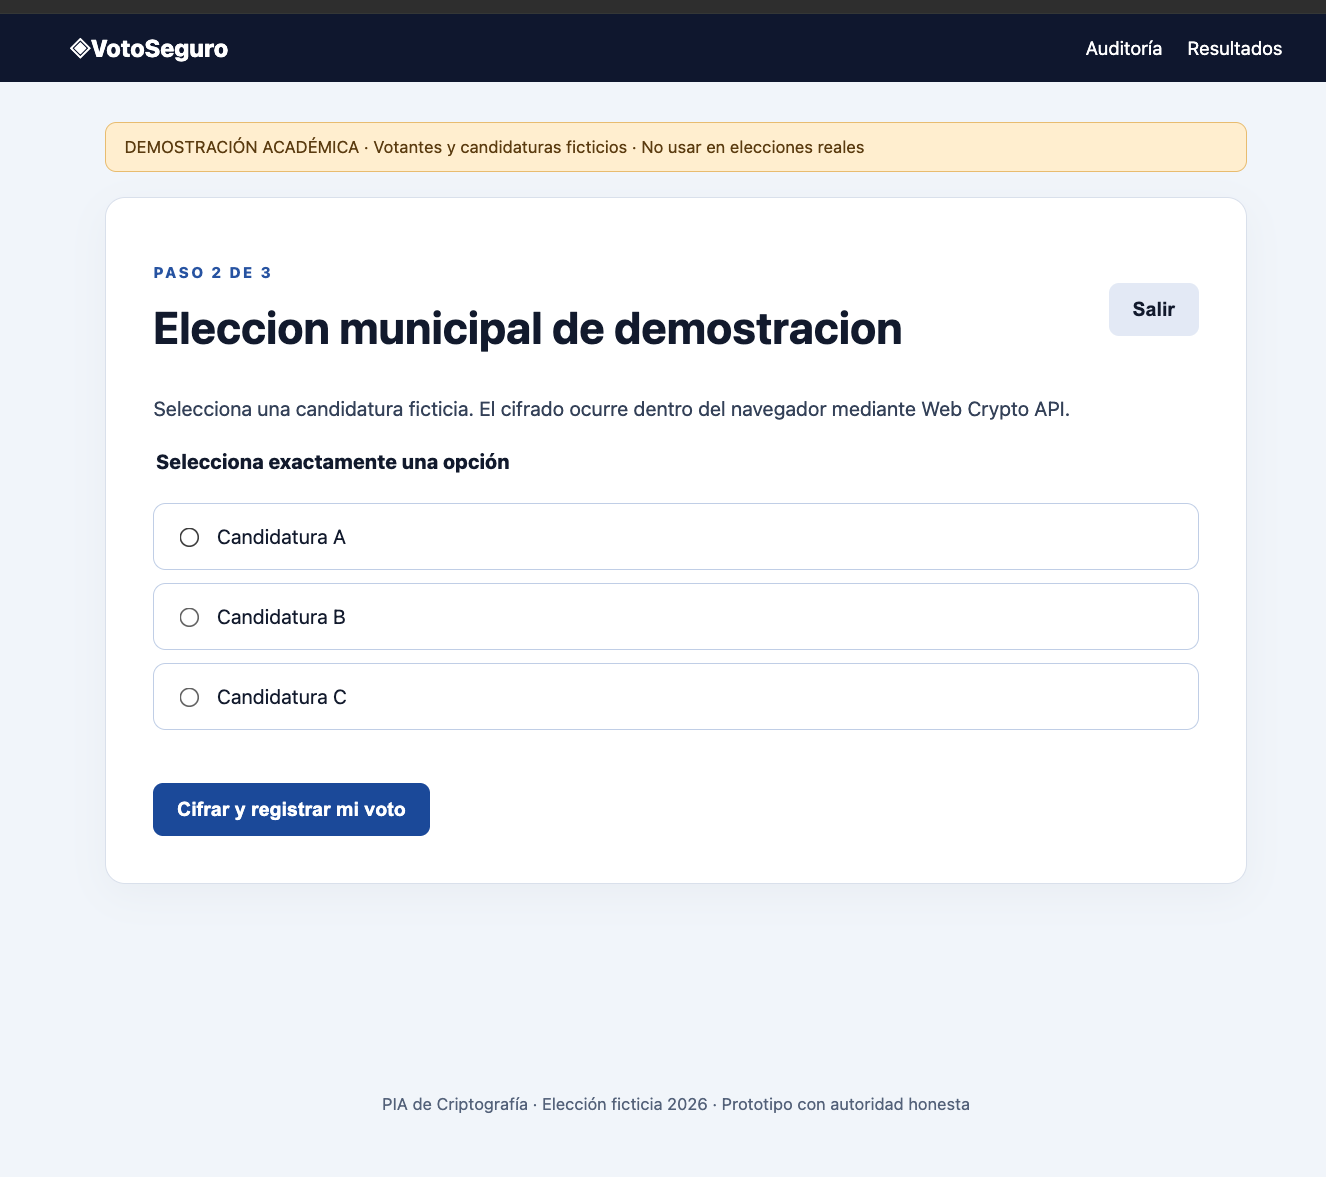
\includegraphics[width=.85\linewidth]{docs/evidencias/Boleta con 3 candidaturas ficticias.png}

\newpage
\textbf{Selección de uno de los 3 candidatos}
\newline
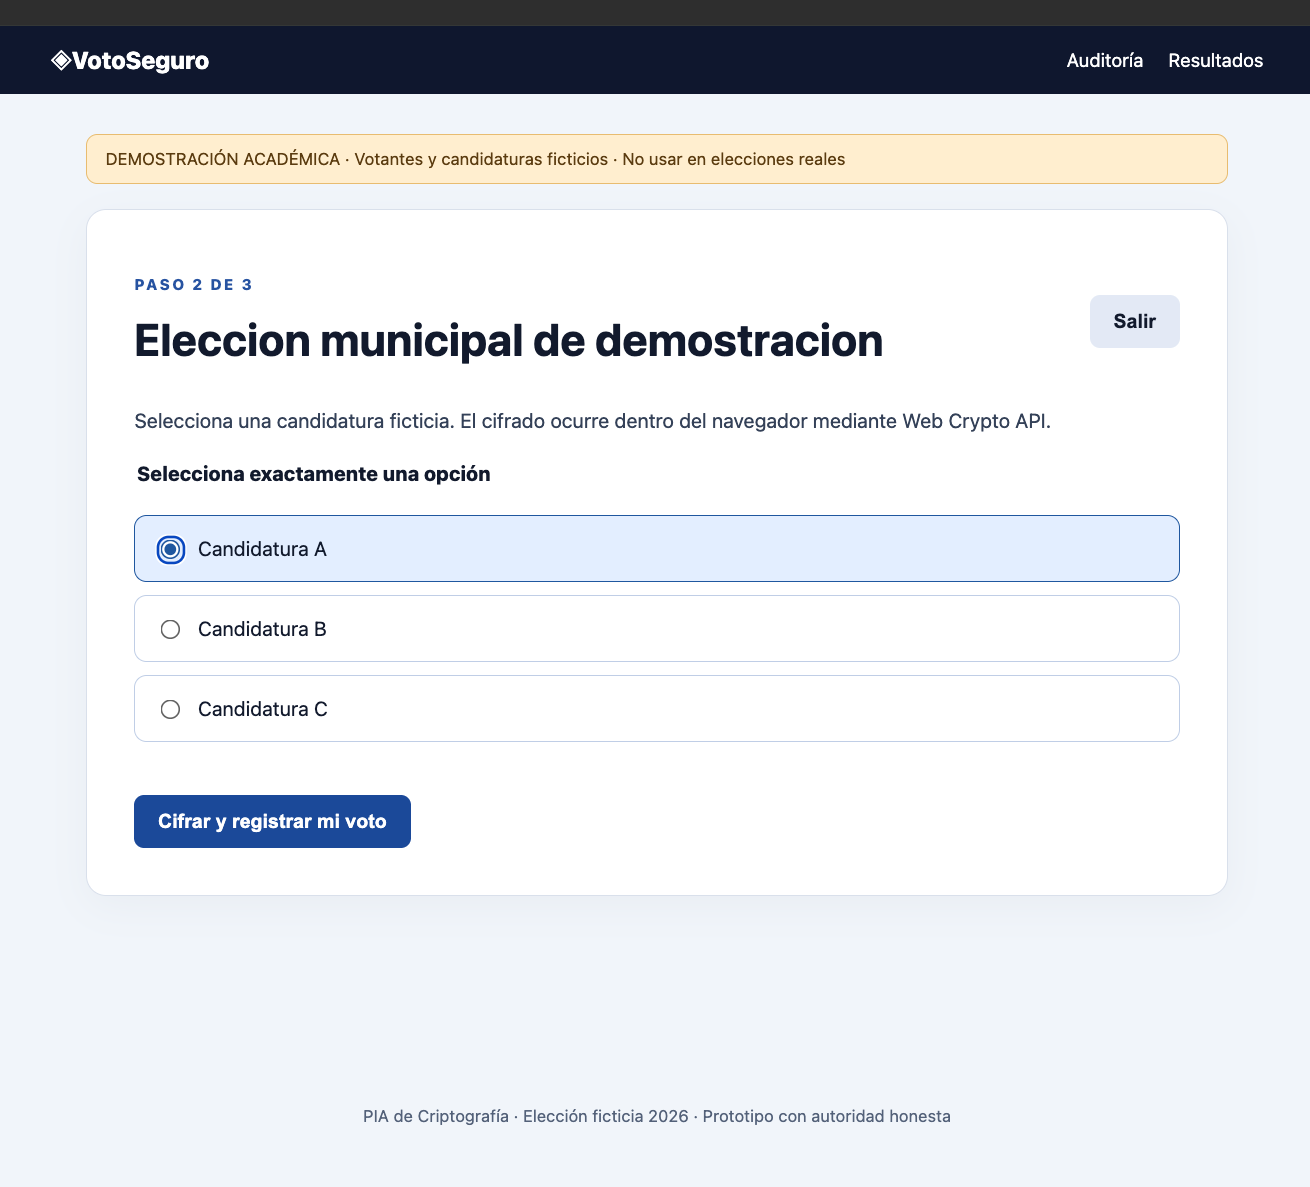
\includegraphics[width=.85\linewidth]{docs/evidencias/Boleta con la candidatura A seleccionada.png}

\newpage
\textbf{Comprobante de registro}
\newline
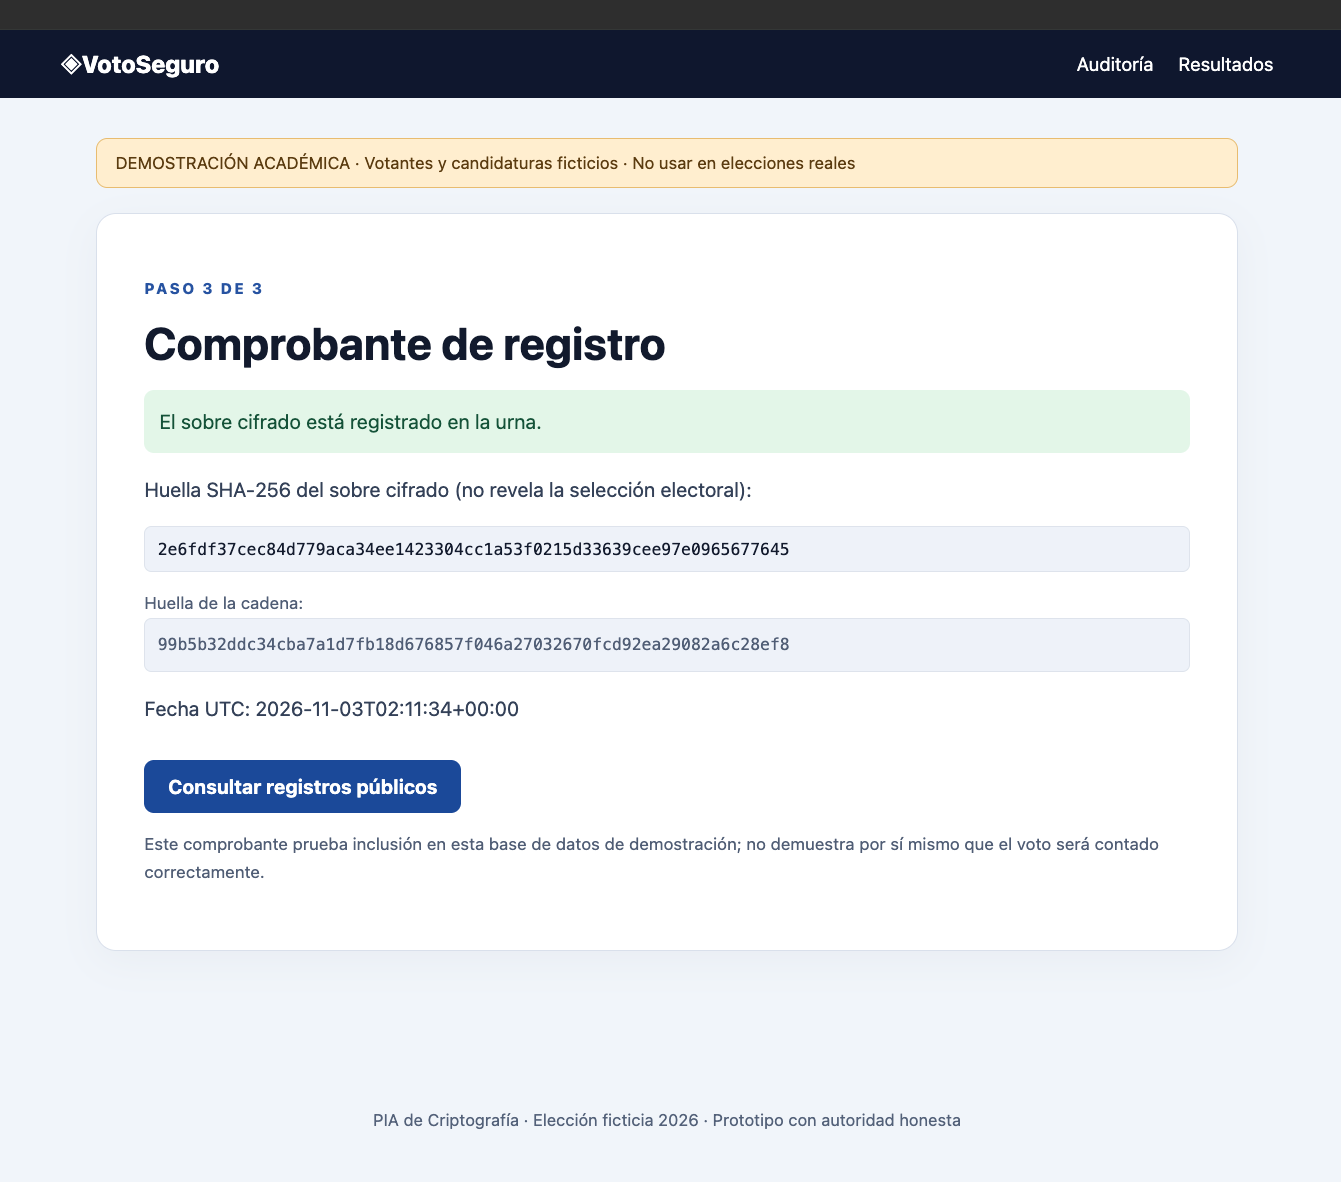
\includegraphics[width=.85\linewidth]{docs/evidencias/Comprobante con voto firmado.png}

\newpage
\textbf{Prohibición al querer votar de nuevo desde una cuenta que ya voto antes}
\newline
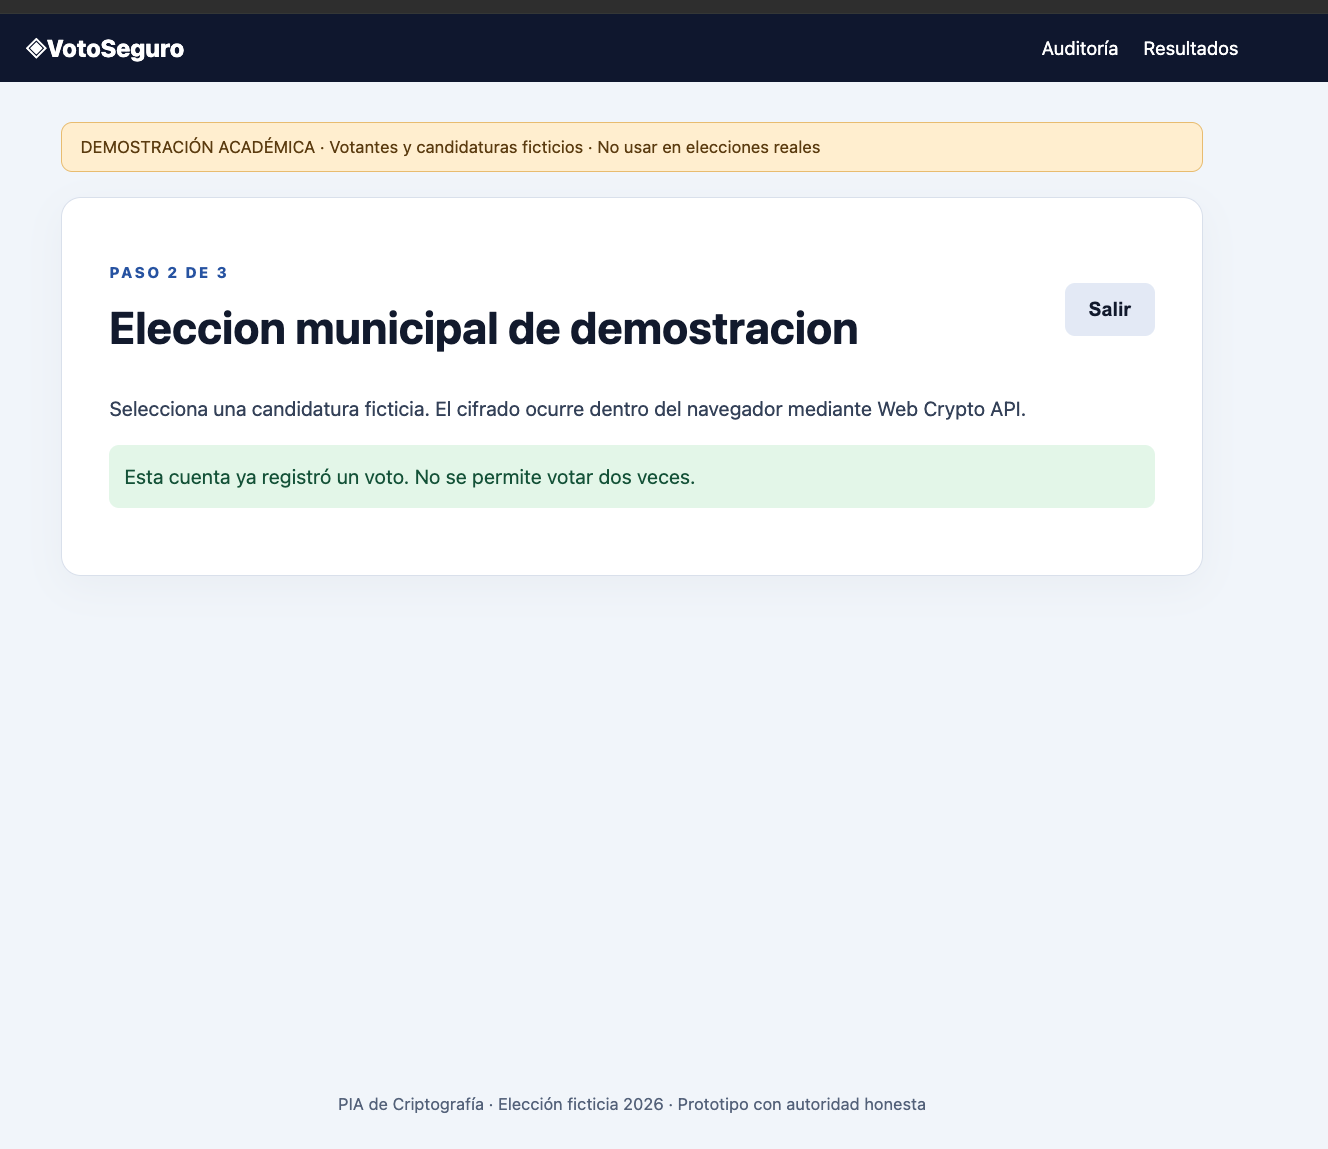
\includegraphics[width=.85\linewidth]{docs/evidencias/Intento rechzado.png}

\textbf{Prueba de escrutinio (urna aun abierta)}
\newline
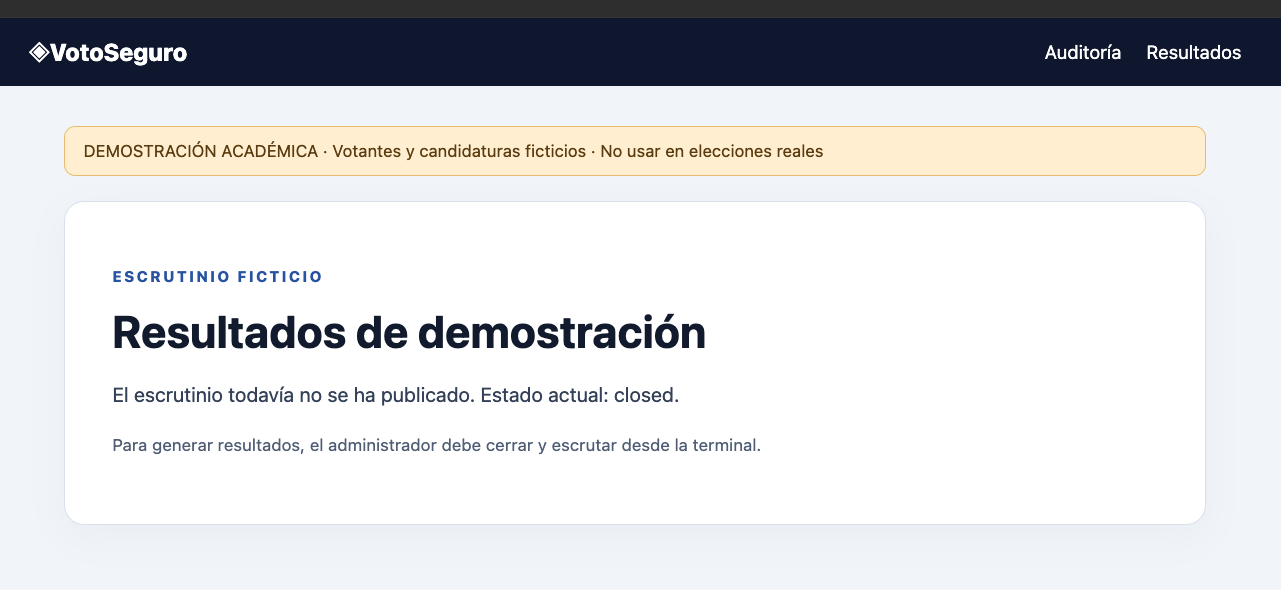
\includegraphics[width=.85\linewidth]{docs/evidencias/urna cerrda.png}

\newpage
\textbf{Prueba de los 5 votos de las 5 cuentas}
\newline
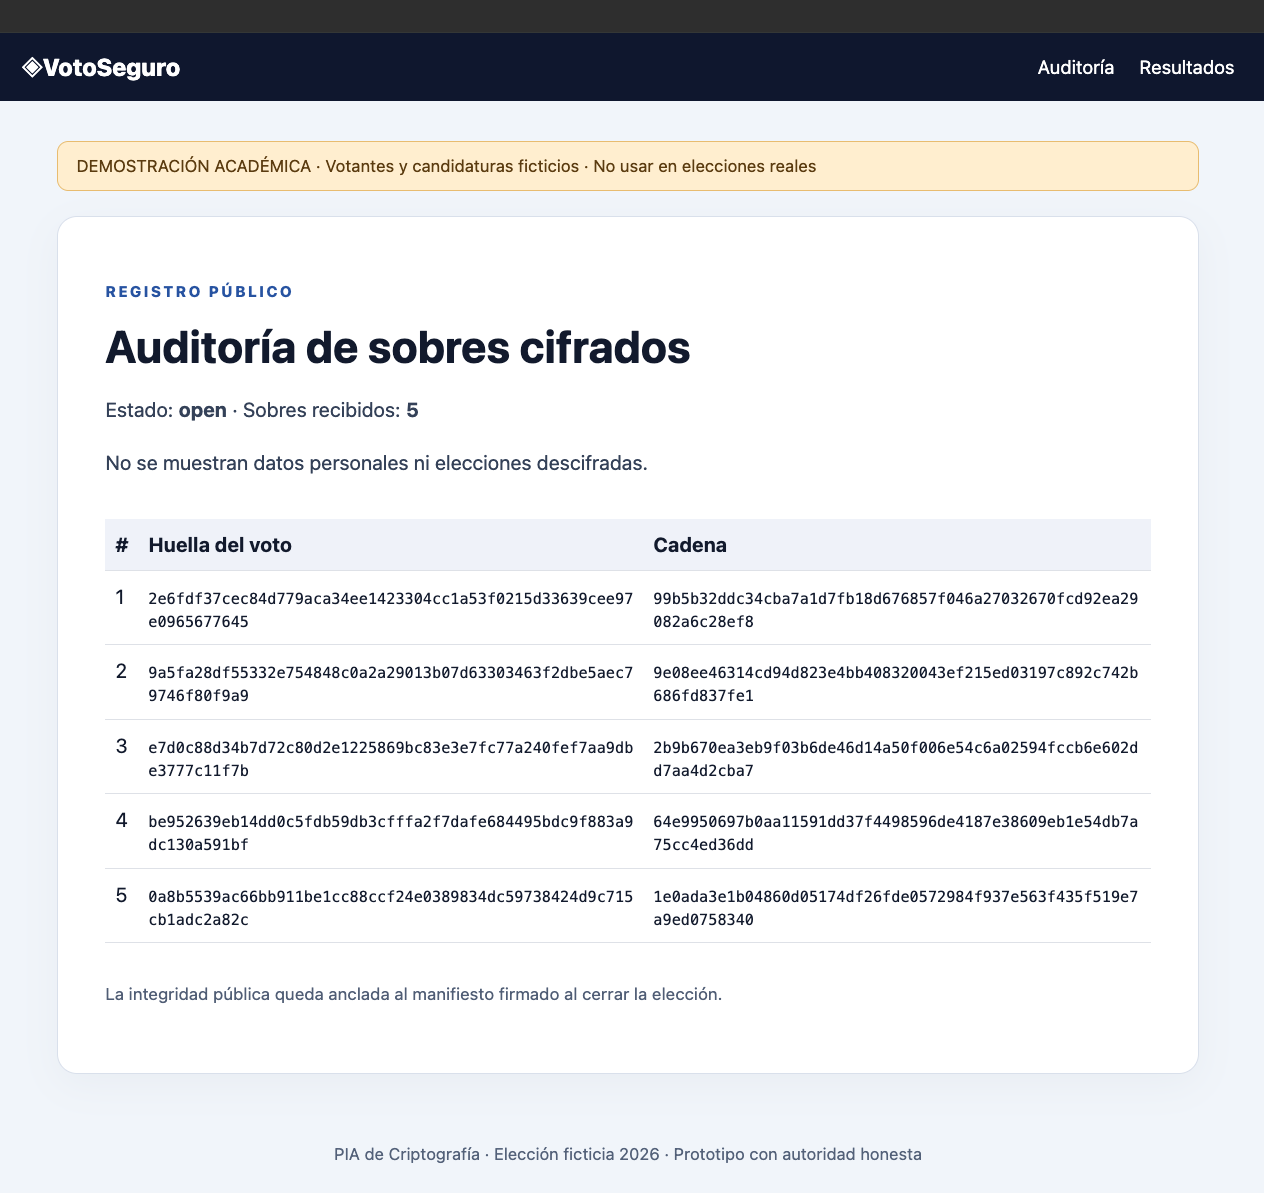
\includegraphics[width=.85\linewidth]{docs/evidencias/5 votos.png}

\newpage
\textbf{Prueba del resultado final}
\newline
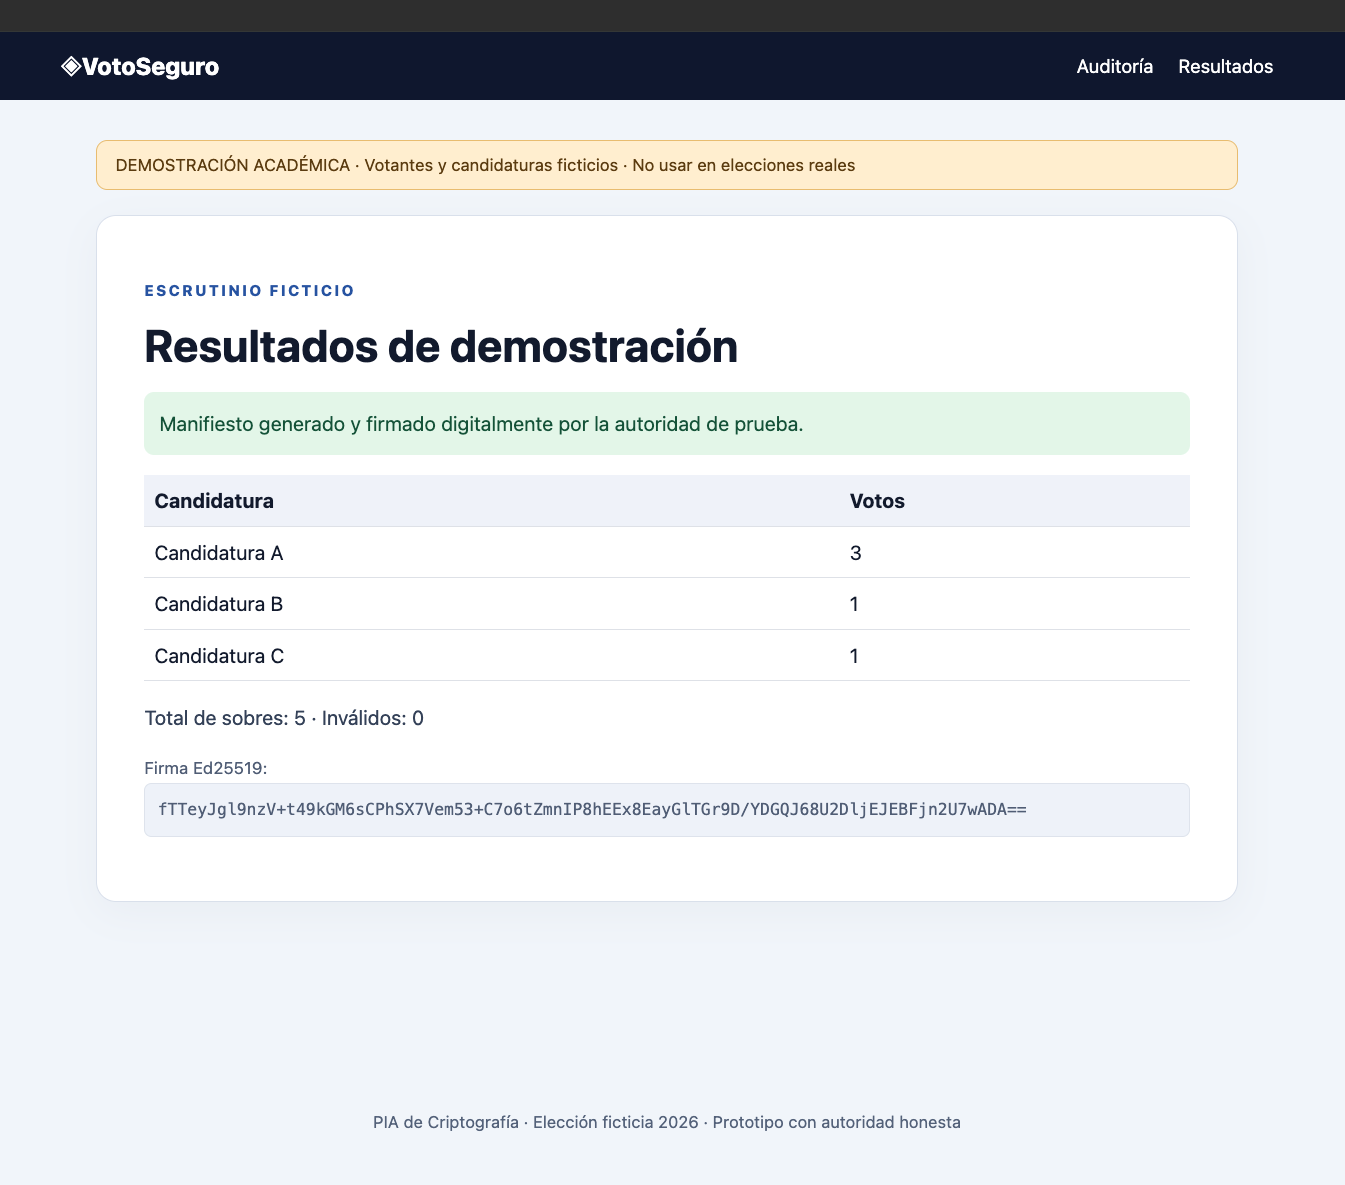
\includegraphics[width=.85\linewidth]{docs/evidencias/Firma final y resultados.png}

\textbf{Prueba de la terminal de comandos y de la validación de cadenas y firma}
\newline
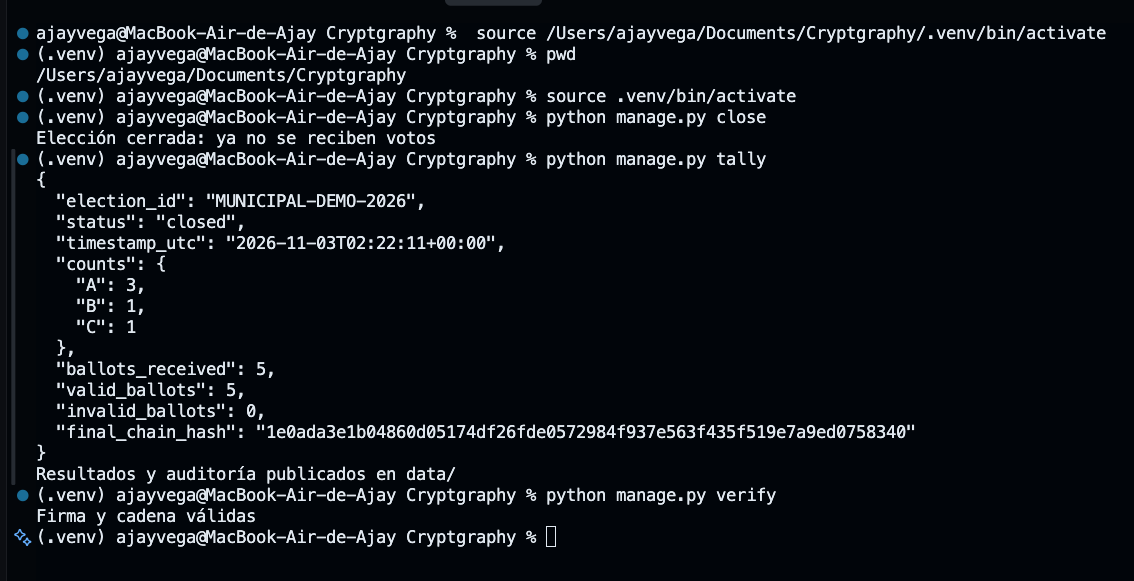
\includegraphics[width=.85\linewidth]{docs/evidencias/Terminal con proceso.png}
%--
%--\missingimage{Formulario de inicio de sesión con usuario ficticio }
%--\missingimage{la boleta y tres candidaturas ficticias}
%--\missingimage{el fckin comprobante SHA-256 de un voto confirmado}
%--\missingimage{y un ntento repetido y rechazo del sistema}
%--\missingimage{la auditoria, resultados y la terminal con pytest}

% NIGGAAA, Para sustituir cada recuadro en Overleaf, subir la captura a la carpeta \code{evidencias/} y reemplazar la instrucción \code{\\missingimage\{...\}} por \code{\\includegraphics[width=.85\\linewidth]\{evidencias/nombre.png\}}.

% nigga thx

\section{Conclusiones}

\subsection{Conclusion general}
VotoSeguro ejemplifica cómo varios mecanismos criptográficos pueden colaborar en un protocolo de votación electrónica simulado. Argon2id protege las contraseñas almacenadas; RSA-OAEP y AES-GCM permiten transmitir un voto en forma cifrada; las transacciones SQLite impiden la duplicación por cuenta; SHA-256 detecta alteraciones del registro encadenado; y Ed25519 autentica el manifiesto final publicado.

La selección de algoritmos depende de su función: el cifrado simétrico es adecuado para el contenido de las boletas, el asimétrico sirve para transportar su clave, los hashes para registrar huellas y las firmas para autenticar resultados. Ningún método por sí solo resuelve todos los requisitos.

El prototipo también permite reconocer límites importantes: una autoridad honesta sigue siendo un supuesto de confianza, no se ha demostrado anonimato completo frente a correlación de metadatos, no existe un mecanismo matemático de escrutinio públicamente verificable y el sistema local no está preparado para una elección oficial. Por tanto, su propósito es \textbf{didáctico y experimental}, no electoral operativo.

\newpage
\subsection{Conclusiones individuales}
\textbf{Axel Ivan Verastegui Patino - 2091219}:
\newline
Al realizar este proyecto nos dimos cuenta de que crear un sistema de votación electrónica seguro es mucho más complicado de lo que parece. Al principio podría pensarse que basta con registrar usuarios y contar votos, pero existen muchos aspectos que debemos considerar, como evitar votos duplicados, proteger las contraseñas y verificar que los resultados no hayan sido alterados. 
Aunque logramos desarrollar un prototipo funcional, entendimos que un sistema utilizado en elecciones reales necesitaría muchas más pruebas, medidas de seguridad y supervisión antes de poder implementarse.\\

\textbf{Julio Cesar Puente Reynoso - 2115192}:
\newline
text.\\

\textbf{Cecilia Ximena Gonzales Chavez - 2069031}:
\newline
bruh.\\

\textbf{Diego Alejandro Puente Ruiz - 2095327}:
\newline
thfck.\\

\textbf{Sebastian Flores Gonzales - 2104564}:
\newline
 more xmore\\

\section*{Referencias bibliográficas}
\addcontentsline{toc}{section}{Referencias bibliográficas}
\begin{thebibliography}{99}
\bibitem{nistvvsg} NIST. \emph{Voluntary Voting System Guidelines: Principles and Guidelines}. \url{https://www.nist.gov/itl/voting/vvsg-principles-and-guidelines}
\bibitem{owasp} OWASP. \emph{Password Storage Cheat Sheet}. \url{https://cheatsheetseries.owasp.org/cheatsheets/Password_Storage_Cheat_Sheet.html}
\bibitem{mdn} MDN Web Docs. \emph{SubtleCrypto API}. \url{https://developer.mozilla.org/en-US/docs/Web/API/SubtleCrypto}
\bibitem{flask} Pallets. \emph{Flask Security Considerations}. \url{https://flask.palletsprojects.com/en/stable/web-security/}
\bibitem{rfc8017} Moriarty et al. \emph{RFC 8017: PKCS \#1 RSA Cryptography Specifications Version 2.2}. \url{https://www.rfc-editor.org/rfc/rfc8017}
\bibitem{nistgcm} NIST. \emph{SP 800-38D: Recommendation for Block Cipher Modes of Operation: GCM and GMAC}. \url{https://doi.org/10.6028/NIST.SP.800-38D}
\bibitem{rfc8032} Josefsson y Liusvaara. \emph{RFC 8032: Edwards-Curve Digital Signature Algorithm (EdDSA)}. \url{https://www.rfc-editor.org/rfc/rfc8032}
\end{thebibliography}

\end{document}
